\chapter{RESULTS}

\label{sec:results_intro}
The NECTA framework functions not merely as an underlying analytical script, but as an integrated, high-performance neuroinformatic tool engineered to ingest high-density electrophysiological data and interactively map time-resolved cortical workflows. Before breaking down the specific statistical topographies of the network, the baseline operational capacity of this developed framework is established. As visualized in Figure~\ref{fig:necta_tool} (previously conceptualized as the framework entry point), the pipeline orchestrates multi-channel inputs to slice the functional connectome millisecond-by-millisecond, overcoming standard computational bottlenecks.

\vspace{1cm}
\begin{figure}[htbp]
    \centering
    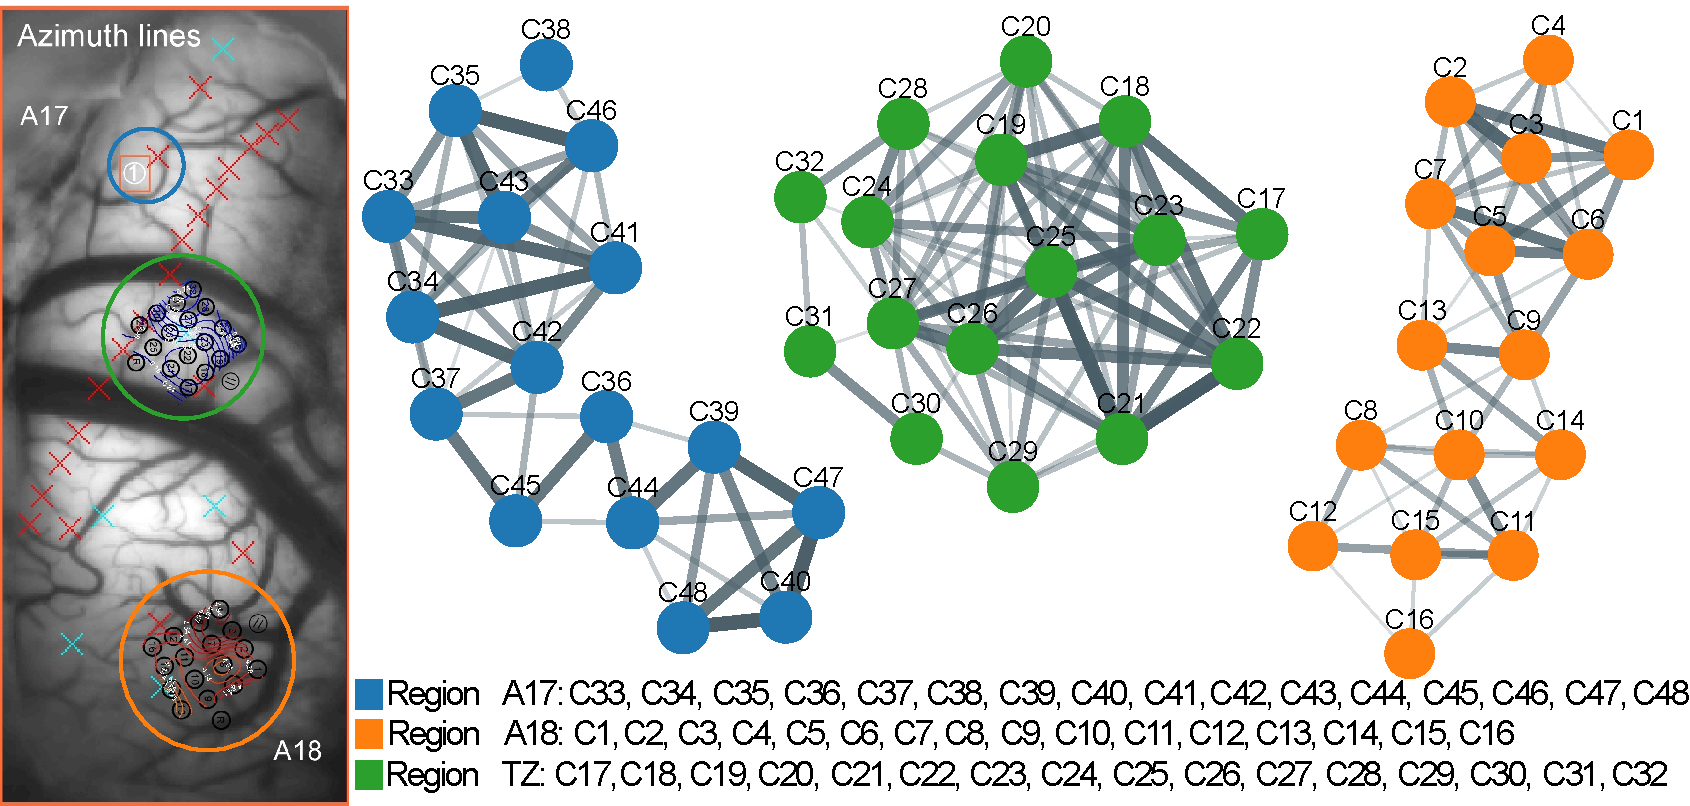
\includegraphics[width=\linewidth]{./figuras/Intro/Figura01.pdf}
    \caption[Mapping directly to the anatomically separated electrode matrixes]{\textbf{Direct Mapping of Coherence Clusters onto Anatomically Separated Electrode Matrices.} Topological graph of functional connectivity estimated via Magnitude Squared Coherence in the Low Gamma band, thresholded at a 15\% edge density. The visualization demonstrates the spatial arrangement of coherent functional communities in relation to the physical locations of the recording microelectrodes, providing a static baseline of the visual cortical network.}
    \label{fig:necta_tool}
\end{figure}
\vspace{1cm}

\section{Baseline Characterization and the Static Backbone}
To establish a baseline structural framework, static functional connectivity was evaluated across the entire recording session. Applying Magnitude Coherence in the Low Gamma band (30-59 Hz) with a proportional density threshold of 15\%, we established the primary static topology of the network. The Louvain community algorithm blindly extracted functional clusters that closely matched the anatomical placement of the multielectrode arrays, naturally partitioning into three distinct topological modules corresponding to Area 17 (A17), the Transition Zone (TZ), and Area 18 (A18). This static connectome serves as the anatomical "structural backbone" \cite{vezoli2021}.

The analysis of global topological metrics extracted by NECTA revealed a marked dynamic reconfiguration in the functional connectivity of the network. As illustrated in Figure \ref{fig:topological_dynamics}(A), both Global Efficiency and the Clustering Coefficient exhibited high variability across time windows, evidencing the non-stationary and volatile character of cortical processing.

More critically, the analysis of the Small-World Index ($\sigma$) (Figure \ref{fig:topological_dynamics}(B)) demonstrated that the network transitions into highly efficient topological optimization states in specific frequency bands. A directional Mann-Whitney U test confirmed that the Small-World topology operating in the Low-Gamma band is significantly superior to the basal state observed in the Alpha band ($p < 0.05$).

The wide dispersion of $\sigma$ values in the Low-Gamma band reveals transient topological surges reaching values above 5.0. These fluctuations demonstrate that the small-world configuration in this frequency range does not maintain a stationary state, but rather alternates between baseline levels and discrete peaks of high network integration.

\section{Time-Resolved Causal Interactions}
A prerequisite for establishing dynamic visual dynome topology is the direct quantification of causal information flow between nodes without the bias of temporal averaging. We utilized the developed NECTA framework to extract the evolution of time-resolved causal coupling using the Partial Directed Coherence (PDC) metric across sensory ingestion epochs.

Figure~\ref{fig:pdc_graph} visualizes these raw directional data. Following stimulus onset (represented by $T=0$), distinct causal spikes appear that define the functional state. Specifically, Striate cortex (A17) drove the initial response to extrastriate targets (e.g., A17$\to$TZ) with a PDC peaking at  752.4~ms relative to stimulus onset, reaching $0.19 \pm 0.13$. This data provides the empirical foundation to move beyond descriptive graph metrics, demonstrating that sensory information flow reconfigures rapidly during the active state, transitioning control from striate to extrastriate sources.

\begin{figure}[htpb]
    \centering
    
\includegraphics[width=\textwidth]{figuras/PDC_graph.pdf}
    \caption[Time-resolved Causal Connectivity derived from the NECTA framework]{The figure displays the evolution of Partial Directed Coherence (PDC) over visual ingestion epochs. Colored lines represent distinct directional area connections (e.g., Blue: A17$\to$TZ; Red: A18$\to$TZ). Spikes in the PDC metric indicate active causal information transfer that redefines the visual dynome topology during active sensory states.}
    \label{fig:pdc_graph}
\end{figure}

\section{Topological Evolution of the Visual Dynome}
By applying graph-theoretical metrics to the matrices derived from the raw causal flow quantified in the preceding section, we visualized the topology of the visual dynome. Figure~\ref{fig:dyna_graphs} illustrates this time-resolved evolution, contrasting distinct sensory processing states.

To understand the relationship between localized neural activity and global network architecture, we analyzed the aggregate spike counts alongside the Small-Worldness ($\sigma$) index across continuous 250 ms sliding windows. As illustrated in Figure~\ref{fig:spike_vs_sw}, the transition from the baseline state to active sensory ingestion triggers a synchronized physiological and topological response.

Following the stimulus onset, a prominent peak in the aggregate spike count is closely accompanied by a pronounced increase in the Small-Worldness index, particularly visible around Window 3 and Window 4. The network consistently maintains a $\sigma > 1$ threshold, confirming that the visual dynome operates within a highly efficient small-world regime. This temporal alignment provides consistent evidence that the visual cortex rapidly shifts towards a highly integrated and segregated topology during periods associated with increased sensory processing.

\begin{figure}[htpb]
    \centering
    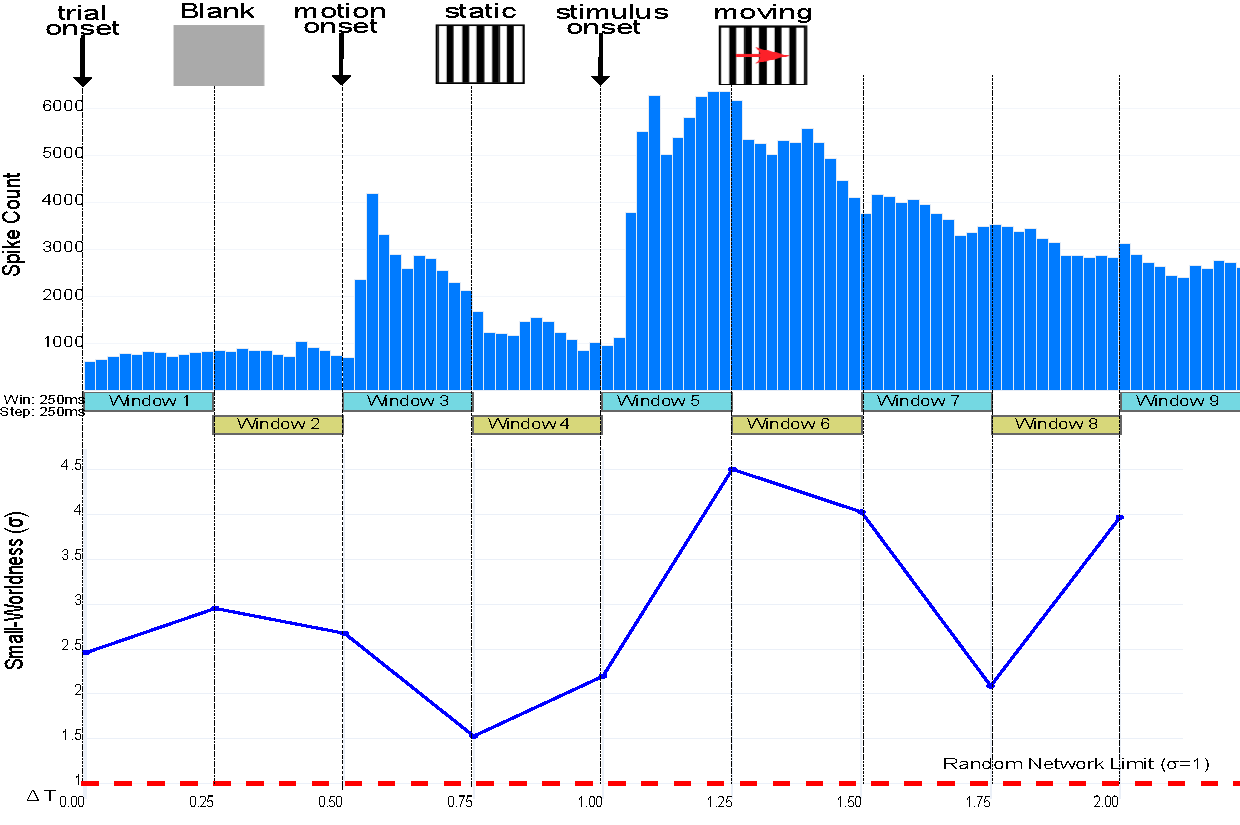
\includegraphics[width=\textwidth]{figuras/SpikeVsSW.pdf}
    \caption[Temporal alignment of localized neural activity and global network topology]{Temporal alignment of localized neural activity and global network topology. (Top) Aggregate spike count across the recorded channels, highlighting the peak firing rate during the active visual motion epoch. (Bottom) Evolution of the Small-Worldness ($\sigma$) index computed over 250 ms sliding windows with a 250 ms step. The network consistently operates above the random network limit ($\sigma = 1$), dynamically optimizing its efficiency in response to sensory ingestion.}
    \label{fig:spike_vs_sw}
\end{figure}

While global metrics such as Small-Worldness indicate an overall optimization in network efficiency, the true complexity of the visual dynome is unmasked by observing the specific topological microstates. By extracting the Maximum Spanning Tree (MST) backbones at a proportional density threshold of 23\%, we can track the specific causal routing pathways milisecond-by-millisecond.

Figure~\ref{fig:dynamic_graphs} visualizes these time-resolved structural reconfigurations across the first six epochs. In the initial windows (0.00s--0.50s), the network exhibits a dense, highly clustered state. However, as the processing demands evolve (e.g., Windows 4 and 5), the topology transitions into transient microstates where specific extrastriate and Transition Zone (TZ) nodes become central communication hubs. This rhythmic pulsation---shifting between dense integration and targeted segregation---demonstrates that the A17-TZ-A18 axis does not rely on a rigid communication structure, but rather forms ephemeral pathways to dynamically route visual information.

\begin{figure}[htpb]
    \centering
    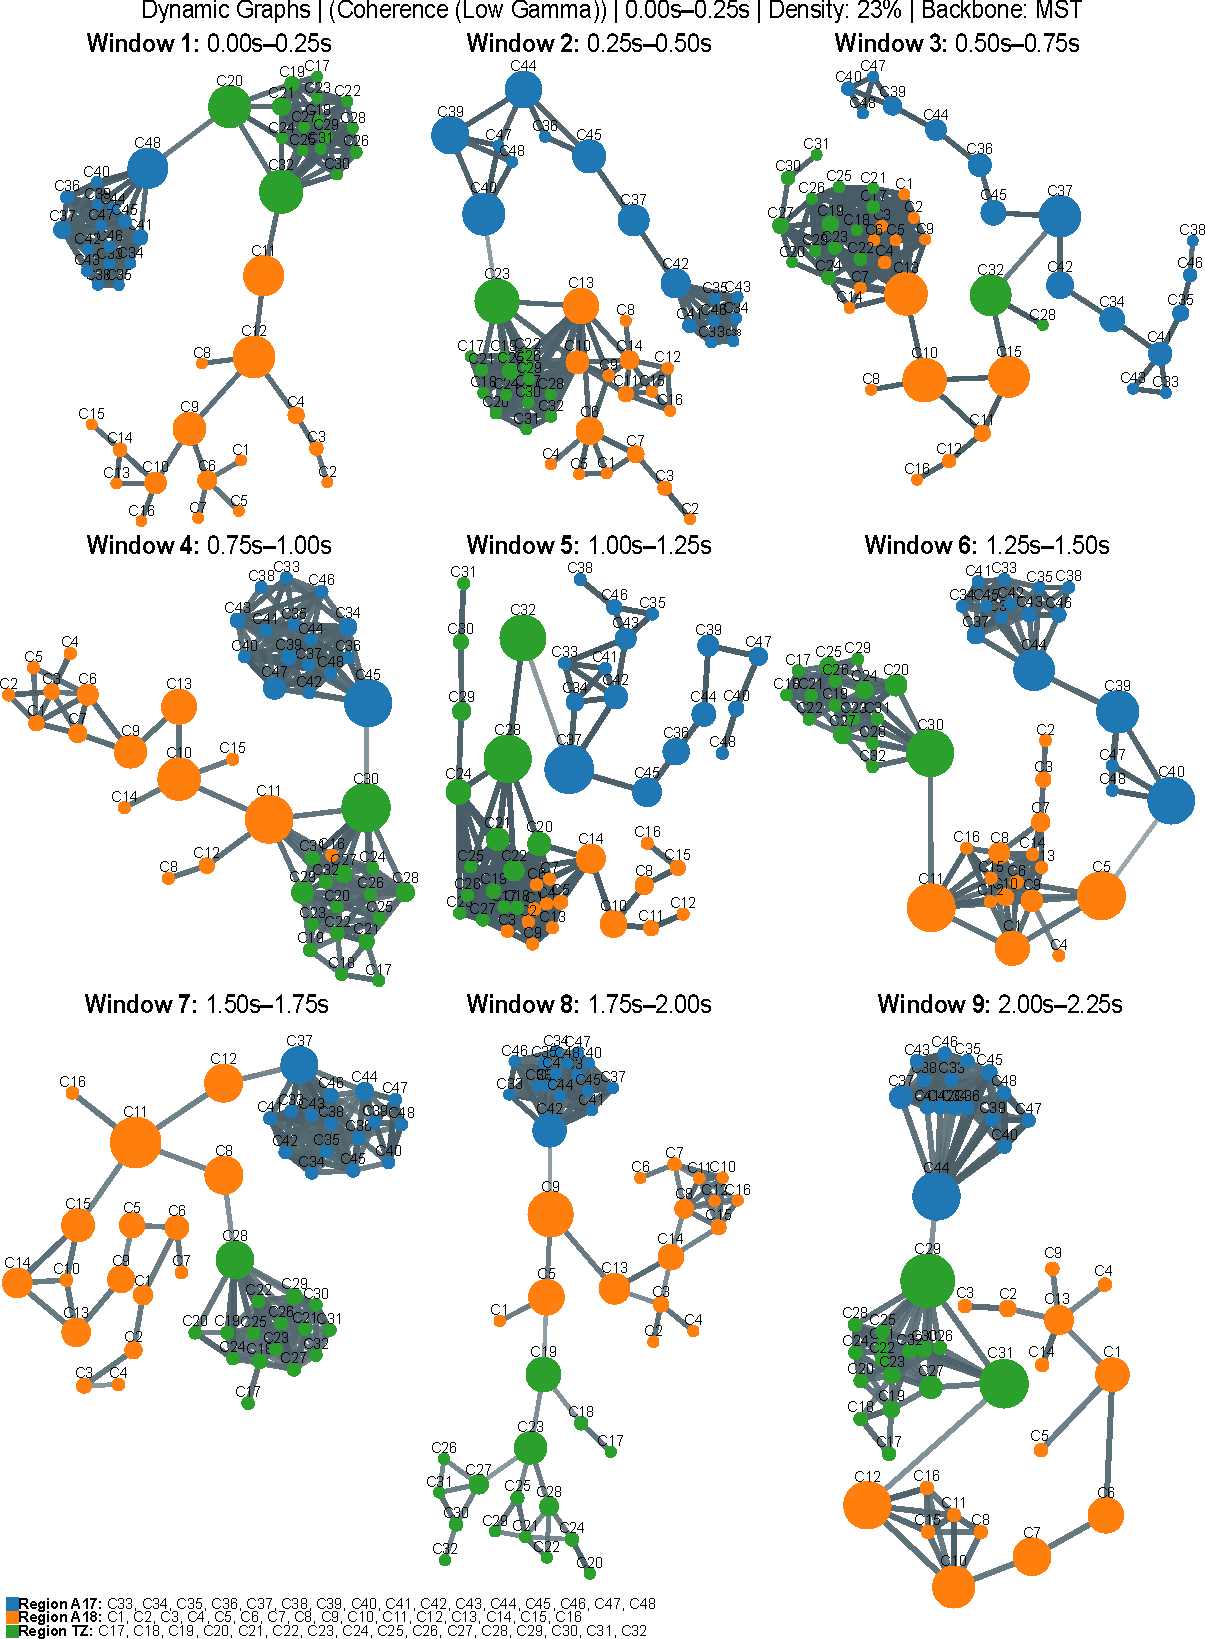
\includegraphics[width=\textwidth]{figuras/Dynamic Graphs.pdf}
    \caption[Time-resolved topological microstates of the visual dynome]{Time-resolved topological microstates of the visual dynome. The sequence illustrates the dynamic graph coherence in the Low Gamma band across 250 ms sliding windows. To highlight the primary routing architecture and eliminate spurious connections, networks are thresholded at 23\% density with a Maximum Spanning Tree (MST) backbone. Node colors correspond to distinct cortical areas: A17 (Blue), Transition Zone (Red), and A18 (Green). The topological volatility confirms the continuous reconfiguration of the cortical hierarchy during active perception.}
    \label{fig:dynamic_graphs}
\end{figure}

\begin{figure}[htbp]
    \centering
    
\includegraphics[width=\textwidth]{Metricas_NECTA.pdf}
    \caption[Topological Dynamics and Small-World Optimization]{\textbf{Topological Dynamics and Small-World Optimization in the Visual Cortex.} \textbf{(A)} High temporal variability of Global Efficiency and Clustering Coefficient. The substantial dispersion (ranging from 0.2 to 0.8) illustrates the volatile dynamics of cortical processing, as the network continuously balances moments of strong local processing (high clustering) with global communication jumps (high efficiency). \textbf{(B)} Comparison of the Small-World Index ($\sigma$) between the Alpha (8-12 Hz) and Low-Gamma (30-59 Hz) bands. The asterisk (*) denotes a statistically significant increase in Small-World topology during Low-Gamma. The pronounced dispersion (elongated whiskers) underscores that the network operates through transient, high-efficiency topological pulses rather than remaining in a static optimized configuration.}
    \label{fig:topological_dynamics}
\end{figure}

To further evaluate the structural hierarchy of the visual network, we investigated the Node Strength of the cortical areas within the Gamma band. The analysis of the empirical distribution revealed markedly distinct connectivity profiles between primary and higher-order areas.

As evidenced in Figure \ref{fig:node_strength}, Area 17 presents a restricted network centrality with low dispersion. The empirical distribution indicates that network integration within the Gamma band is concentrated in the A18-TZ axis, while A17 remains at the structural periphery.

A defining feature of this functional axis is the bimodal signature evident in the raw scatter distributions of both Area 18 and the Transition Zone. The individual data points do not cluster homogeneously around the median; rather, they segregate into two distinct topological regimes: a basal state of low connectivity (clustering near a Node Strength of 5) and discrete surges of substantial systemic integration (reaching values near 30). This pronounced bimodality reveals that the functional architecture is not a stationary state but a highly dynamic mechanism. The network effectively operates in discrete bursts, with the TZ and A18 transiently exhibiting increased hub-like properties to coordinate stimulus processing, before subsequently relaxing into a decoupled state.

Furthermore, the Transition Zone displays a Node Strength visibly superior to that of Area 18. At a proportional density threshold of 15\% in the Low Gamma band, the Transition Zone (TZ) exhibited a Node Strength ($M = 9.60$, $SD = 3.50$), compared to A18 ($M = 7.25$, $SD = 3.11$). The statistical analysis revealed a significant difference between the regions (Mann-Whitney $U = 186.0$, $p = 0.030$, effect size $r = 0.453$). This demonstrates that the Transition Zone operates under a connectivity load that statistically surpasses Area 18.

\begin{figure}[htbp]
    \centering
    
\includegraphics[width=\textwidth]{Forca_Nodal_TZ.pdf}
    \caption[Node Strength Distribution in the Gamma Band]{\textbf{Node Strength Distribution in the Gamma Band.} Area 17 displays restricted centrality with low variability. In contrast, both the Transition Zone (TZ) and Area 18 exhibit bimodal distributions with high variability. The Transition Zone operates under a connectivity load tendentially superior to that of Area 18, highlighting its role as a primary interhemispheric convergence hub.}
    \label{fig:node_strength}
\end{figure}

\section{Hierarchical Information Flow (Directed Connectivity)}
To decode the causal relationships within this structural backbone, Partial Directed Coherence (PDC) was applied using the BIC-optimized MVAR models. The static PDC analysis in the Low Gamma band revealed a highly asymmetrical and hierarchical information flow across the visual cortex. 
By calculating the Net Flow for each region, the analysis indicates that A17 behaves as the dominant persistent Driver, exhibiting a significantly higher Net Flow ($M = 1.21$, $SD = 1.17$) compared to the rest of the network ($M = -0.60$, $SD = 1.37$; Mann-Whitney $U = 424.0$, $p = 1.245 \times 10^{-4}$, effect size $r = -0.656$). In contrast, A18 behaves as the primary \textit{Receiver} (Sink) (-1.36 net flow). These results suggest a directional pathway extending from A17 through the TZ and terminating in A18 (A17 $\rightarrow$ TZ $\rightarrow$ A18).

\section{Dynamic Topology and Temporal Integration}
The core capability of NECTA lies in capturing the time-varying network dynamics—the transition from static networks to chronological connectomes. Connectivity was recalculated using a sliding-window approach ($W = 500$ ms, 50\% overlap). The Temporal Integration panel overlaid the global population spiking activity (Peri-Stimulus Time Histogram - PSTH) with the topological evolution of the network's \textit{Small-Worldness} ($\sigma$).

The dynamic analysis revealed that the network's topological efficiency is not static but responds to visual processing phases. The network achieved its absolute peak in \textit{Small-Worldness} specifically during the moving grating stimulus phase. This transient optimization was driven primarily by a rapid surge in local clustering, indicating that the cortical network reorganizes into a highly efficient state to process dynamic visual inputs.

\vspace{1cm}

% --- VISUAL INSERTION 3 USING TIKZ ---
\begin{figure}[htbp]
    \centering
    \begin{tikzpicture}[
        >=Stealth,
        node distance=3.5cm,
        area/.style={circle, draw, minimum size=1.5cm, font=\sffamily\bfseries, thick, align=center},
        source/.style={fill=red!20, draw=red!80!black},
        sink/.style={fill=blue!20, draw=blue!80!black},
        mod/.style={fill=purple!20, draw=purple!80!black},
        neutral/.style={fill=gray!10, draw=gray},
        strongflow/.style={->, ultra thick, draw=red!70!black},
        weakflow/.style={->, thick, dashed, draw=gray},
        activeflow/.style={->, line width=2.5pt, draw=orange!90!black}
    ]

    % --- PANEL A: Baseline ---
    \node[font=\sffamily\bfseries] at (0, 3) {Panel A: Baseline Period (Silent Pre-Stimulus)};
    
    \node[area, source] (A17_A) at (-3, 0) {A17\\(+ Net)};
    \node[area, neutral] (TZ_A) at (0, -2) {TZ\\(Neutral)};
    \node[area, sink] (A18_A) at (3, 0) {A18\\(- Net)};
    
    % Flows for Panel A
    \draw[strongflow] (A17_A) -- node[above, font=\sffamily\scriptsize] {Dominant Driver} (A18_A);
    \draw[weakflow] (A17_A) -- (TZ_A);
    \draw[weakflow] (TZ_A) -- (A18_A);
    
    \node[font=\sffamily\scriptsize, text=gray!80!black, align=center] at (0, -3.2) {Chronic Resting Flow:\\ Hierarchy A17 $\rightarrow$ A18};

    % --- PANEL B: Stimulus Peak ---
    \begin{scope}[yshift=-7.5cm]
        \node[font=\sffamily\bfseries] at (0, 3) {Panel B: Modular Peak (\textit{Grating} Onset)};
        
        \node[area, source] (A17_B) at (-3, 0) {A17\\(Source)};
        \node[area, mod, fill=orange!30, draw=orange!80!black] (TZ_B) at (0, -2) {TZ\\(Active)};
        \node[area, sink] (A18_B) at (3, 0) {A18\\(Sink)};
        
        % Flows for Panel B
        \draw[strongflow, line width=1.5pt] (A17_B) -- (A18_B);
        \draw[activeflow] (TZ_B) -- node[left=0.2cm, font=\sffamily\scriptsize, align=right] {Directional\\Inversion} (A17_B);
        \draw[activeflow] (TZ_B) -- node[right=0.2cm, font=\sffamily\scriptsize, align=left] {Intense\\Modulation} (A18_B);
        
        \node[font=\sffamily\scriptsize, text=orange!80!black, align=center] at (0, -3.2) {Mutable Polarity:\\ TZ coordinates spatial integration};
    \end{scope}

    \end{tikzpicture}
    \caption[Evolutionary Mapping of Net Flow]{\textbf{Evolutionary Topological Mapping of Information Net-Flow (Low-Gamma Band).} In-degree minus out-degree proportions. \textbf{(A)} During the baseline period, the network operates in a predominant predictive visual hierarchy, where Area 17 (A17) is the primary driving pole and Area 18 (A18) the passive sink, with the Transition Zone (TZ) in a neutral state. \textbf{(B)} At the precise moment of the stimulus (moving \textit{grating} onset), the topology undergoes active remodeling. The TZ reverses its passive polarity and adopts acute modulation dynamics, drastically altering the \textit{edge weights} (arrow thickness) and suggesting that mesoscopic flexibility reacts transiently to the peripheral stimulus input.}
    \label{fig:netflow_evolution}
\end{figure}

\vspace{0.5cm}

\section{Network Evolution and Modulatory Nodes}
Extracting frame-by-frame snapshots (Connectome Filmstrip) of the dynamic Low Gamma Coherence network illustrated a stable rhythmic organization over time. The hubs located in A17 and the TZ maintained cohesive clustering. Crucially, evaluating the \textit{Net Flow Evolution} uncovered a complex temporal interplay obscured by static analysis. While A17 consistently acted as a "Volatile Source" and A18 as a "Stable Sink", the Transition Zone (TZ) exhibited unique behavior. The TZ functioned as a \textit{Dynamic Modulator}, actively switching its directional role (from sink to source, or vice versa) precisely at the onset of visual stimulation. This highlights the framework's capacity to dissect the mesoconnectome chronologically, revealing dynamic hierarchical relays that coordinate sensory integration across the interhemispheric boundary.